\documentclass[letterpaper,11pt]{memoir}
  \usepackage[absolute]{textpos}
  \usepackage{fontspec,graphicx}

  \setsansfont[Scale=1.0,Numbers=OldStyle]{Myriad Pro}

\begin{document}

\frontmatter

\pagestyle{empty}

\textblockorigin{0mm}{0mm}
\setlength{\parindent}{0mm}

\begin{textblock*}{216mm}(0mm,0mm)
  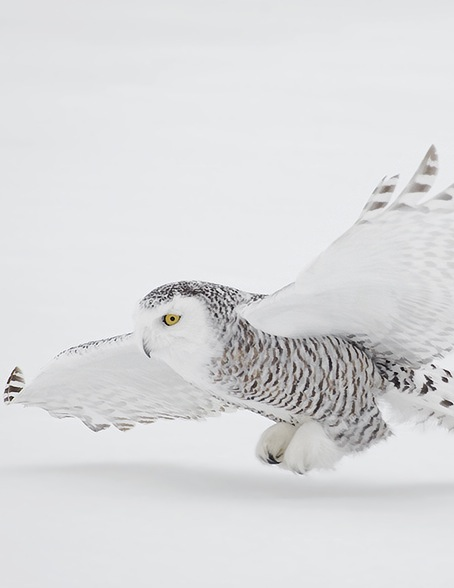
\includegraphics[height=11in,keepaspectratio=true]{harfang.jpg} \\
\end{textblock*}

\begin{textblock*}{176mm}(20mm,35mm)
  \sffamily
  \bfseries\fontsize{42}{42}\selectfont
  %\rule{\linewidth}{0.5pt}
  Introduction à la \\
  programmation en R
  %\rule{\linewidth}{0.5pt}
\end{textblock*}

\begin{textblock*}{176mm}(20mm,75mm)
  \sffamily
  \fontsize{24}{24}\selectfont
  Vincent Goulet
\end{textblock*}

\mbox{}

\newpage

\begin{textblock*}{93mm}[1,0](216mm,0mm)
  
\includegraphics[height=11in,keepaspectratio=true]{harfang-arriere.jpg} \\
\end{textblock*}

\begin{textblock*}{123mm}[0,0](10mm,240mm)
  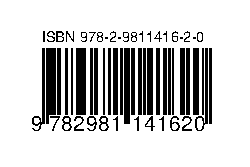
\includegraphics[keepaspectratio=true]{codebarre} \\
\end{textblock*}

\end{document}

%%% Local Variables:
%%% mode: latex
%%% TeX-engine: xetex
%%% TeX-master: t
%%% End:
